% ===========================================
% Template for ICMC 2016 (version2)
% adapted from earlier LaTeX paper templates for the ICMC, SMC, etc...
% ===========================================

\documentclass{article}
\usepackage[utf8]{inputenc}
\usepackage{icmc2016template}
\usepackage{times}
\usepackage{ifpdf}
\usepackage{soul}
\usepackage[english]{babel}
\usepackage{listings}
%\usepackage{cite}


%%%%%%%%%%%%%%%%%%%%%%%% Some useful packages %%%%%%%%%%%%%%%%%%%%%%%%%%%%%%%
%%%%%%%%%%%%%%%%%%%%%%%% See related documentation %%%%%%%%%%%%%%%%%%%%%%%%%%
%\usepackage{amsmath} % popular packages from Am. Math. Soc. Please use the 
%\usepackage{amssymb} % related math environments (split, subequation, cases,
%\usepackage{amsfonts}% multline, etc.)
%\usepackage{bm}      % Bold Math package, defines the command \bf{}
%\usepackage{paralist}% extended list environments
%%subfig.sty is the modern replacement for subfigure.sty. However, subfig.sty 
%%requires and automatically loads caption.sty which overrides class handling 
%%of captions. To prevent this problem, preload caption.sty with caption=false 
%\usepackage[caption=false]{caption}
%\usepackage[font=footnotesize]{subfig}

% ====================================================
% ================ Define title and author names here ===============
% ====================================================
%user defined variables
\def\papertitle{Graphical Temporal Structured Programming for Interactive Music}
\def\firstauthor{Anonymized}
\def\secondauthor{Anonymized}
\def\thirdauthor{Anonymized}

%\def\firstauthor{Jean-Michaël Celerier}
%\def\secondauthor{Myriam Desainte-Catherine}
%\def\thirdauthor{Jean-Michel Couturier}

% adds the automatic
% Saves a lot of output space in PDF... after conversion with the distiller
% Delete if you cannot get PS fonts working on your system.

% pdf-tex settings: detect automatically if run by latex or pdflatex
\newif\ifpdf
\ifx\pdfoutput\relax
\else
   \ifcase\pdfoutput
      \pdffalse
   \else
      \pdftrue
  \fi
\fi

\ifpdf % compiling with pdflatex
  \usepackage[pdftex,
    pdftitle={\papertitle},
    pdfauthor={\firstauthor, \secondauthor, \thirdauthor},
    bookmarksnumbered, % use section numbers with bookmarks
    pdfstartview=XYZ % start with zoom=100% instead of full screen; 
                     % especially useful if working with a big screen :-)
   ]{hyperref}
  %\pdfcompresslevel=9

  \usepackage[pdftex]{graphicx}
  % declare the path(s) where your graphic files are and their extensions so 
  %you won't have to specify these with every instance of \includegraphics
  \graphicspath{{./figures/}}
  \DeclareGraphicsExtensions{.pdf,.jpeg,.png}

  \usepackage[figure,table]{hypcap}

\else % compiling with latex
  \usepackage[dvips,
    bookmarksnumbered, % use section numbers with bookmarks
    pdfstartview=XYZ % start with zoom=100% instead of full screen
  ]{hyperref}  % hyperrefs are active in the pdf file after conversion

  \usepackage[dvips]{epsfig,graphicx}
  % declare the path(s) where your graphic files are and their extensions so 
  %you won't have to specify these with every instance of \includegraphics
  \graphicspath{{./figures/}}
  \DeclareGraphicsExtensions{.eps}

  \usepackage[figure,table]{hypcap}
\fi

%setup the hyperref package - make the links black without a surrounding frame
\hypersetup{
    colorlinks,%
    citecolor=black,%
    filecolor=black,%
    linkcolor=black,%
    urlcolor=black
}

\title{\papertitle}

%\threeauthors
%   {0.5in}
%   {\firstauthor} {LaBRI, Blue Yeti \\ %
 %    {\tt \href{mailto:author1@smcnetwork.org}{author1@smcnetwork.org}}}
 %  {\secondauthor} {LaBRI, CNRS \\ %
  %   {\tt \href{mailto:author2@smcnetwork.org}{author2@smcnetwork.org}}}
  % {\thirdauthor} { Blue Yeti \\ %
   %  {\tt \href{mailto:author3@smcnetwork.org}{author3@smcnetwork.org}}}

\begin{document}
%
\capstartfalse
\maketitle
\capstarttrue
%
\begin{abstract}
     The development and authoring of interactive music or applications, such as user interfaces for arts \& exhibitions
     has traditionally been done with tools that pertain to two broad metaphors. 
     Cue-based environments work by making groups of parameters and sending them to remote devices, 
     while more interactive applications are generally written in generic art-oriented 
     programming environments, such as Max/MSP, Processing or OpenFrameworks.
     In this paper, we argue about the specific issues that arise in such environments, and we present 
     the current version of the i-score sequencer. It is an extensive software suite that bridges
     the gap between time-based, logic-based and flow-based interactive application authoring tools. 
     This is done in a single cohesive graphical user interface, built upon a few simple and novel primitives that give to the composer the expressive power of structured programming, in a time line adapted to the notation of parameter-oriented interactive music.    
\end{abstract}
%

\section{Introduction}\label{sec:introduction}

\section{Temporal multimedia programming}\label{sec:page_size}
\cite{ackermann1994direct}\cite{song1999interactive}
- voir mails envoyés à théo, myriam, etc.
- langages visuels
- références anciens articles i-score 
- protocoles ?
- dire qu'il n'y a pas directement de support des données musicales.

\section{Syntax}
The syntax and graphical elements used in i-score as well as the 
execution semantics are for the most part introduced in \cite{celerier2015ossia, baltazar2014score}.
Multiple execution semantics for the same graphical formalism exist. 
They are based on Petri Nets, Time Automata and Reactive languages.

The novelty lies in the introduction of temporal loops, and of a computation model 
based on Javascript. These two features allow complete expressive power in the 
written scores.

\subsection{Variables}
Variables can be easily implemented by 
- Variables ? 
-> can be stocked in the tree
-> no notion of scope
- JS can be used for local variable concept
\subsection{Temporal structured programming}
\begin{figure}
    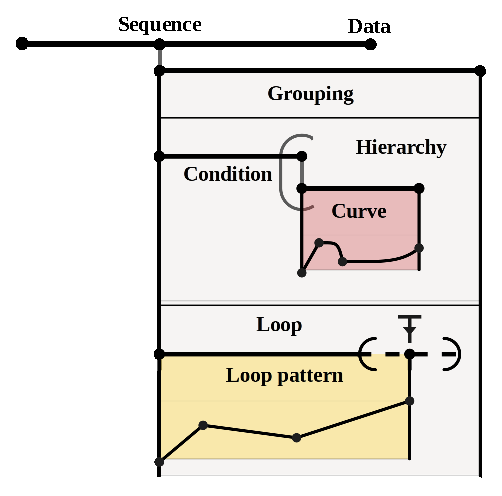
\includegraphics[width=0.45\textwidth]{images/hierarchy.eps}
    \caption{Screenshot of a part of i-score, showing major elements of the formalism.}
    \label{fig.hierarchy}
\end{figure}
Structured programming is a programming paradigm which traces 
back to the 60's, and was conceived at a time where the use of \verb|GOTO|
instructions was prevalent in computing, which often led to code difficult to understand.

The structured programming theorem\cite{bohm1966flow,mills1972mathematical} states that any computable function can be computed 
without the use of \verb|GOTO| instructions, if instead the following operations are available : 
\begin{itemize}
    \item Sequence (\verb|A| followed by \verb|B|), 
    \item Conditional (\verb|if(Pred) then A else B|), 
    \item Iterative (\verb|while(Pred) do A|).
\end{itemize}

Additionnaly, the ability to perform computations is required in order to have a meaningful program.

In order to allow for interactive musical scores authoring, we simulate these concepts in the time-line paradigm.
A virtual machine ticks a timer and makes the time flow in the score graph. 
During this time, multiple processes, which include scenarisation, looping, and multimedia processes, are 
run at each tick. 

Processes can be of two kinds : temporal or instantaneous.
Temporal processes can be explained as functions of time that the composer wants to run between 
two points in time. 
For instance : \emph{do a volume fade-in from t=10s to t=25s}.~\\
Instantaneous processes are functions that will be run at a single point in time.
For instance : \emph{send a single random number to an OSC address}.

Some elements of the syntax are shown in fig.~\ref{fig.hierarchy}.

The scenario is an organisation of the elements of our formalism which allows for sequencing elements, conditional branching, and interactive triggering.
The loop is another organization of the same elements, more restrictive, and with a different control flow.

The software communicates via OSC and maintains a tree of parameters able to mirror 
the object model of remote software built with Max/MSP, PureData, Unity3D or any OSC-compliant environment. 
Conditions, interactive triggers, and more generally all processes of i-score have unrestricted 
access to this tree, and can read its data, perform computations on it, and write it back to the 
remote software.

\section{Authoring features}
i-score provides multiple authoring features aiming to allow 
the composer to express himself.
Besides, the software is based on a plug-in architecture which 
allows for easy extension of its capabilities.
\begin{itemize}
\item Javascript support : one can use Javascript scripts both as temporal and instantaneous processes.
When writing a temporal process, the composer has to provide a function of the form : 
\begin{lstlisting}
function(t) {      
    var obj = new Object; 
    obj["address"] = '/an/osc/address'; 
    obj["value"] = 42; 
 return [ obj ]
}
\end{lstlisting}
When writing an instantaneous process, the function to provide is similar, but does not take the time in argument.
Functions writer are encouraged to write stateless functions, since it would allow for optimizations opportunities such as precomputing an array of values.

\item Automation : the traditional DAW automation, which writes in a parameter over time. Currently provided are 1D (linear, power) and 3D (cubic spline) automations.
\item Mapping : similar in appearance to the automation, this process will take an OSC address as input, apply a transfer function, and write the output to another address.
\item Recording : one can record either automations which will be able to apply automatic interpolation for numeric parameters, or record any kind of input message to replay it afterwards.
\item Execution speed control : the temporal constraints all have a multiplicating coefficient for execution speed.
\item Introspectability : i-score exposes the current score in the same tree that the remote devices. 
Multiple attributes can be queried, and to some extent modified during the execution of the score. 
For instance, the current position of the play head, the activation status of interactive triggers, and the execution speed of all the temporal constraints are controlable parameters.
The elements are organized hierarchically according to their hierarchy in the scenario, and can also be controled from the network.
Plug-ins can expose their own attributes in this tree.
\item Interactive execution : during the authoring process, it is sometimes necessary to replay just a part of the score.
i-score provides this capacity. 
However, it is necessary for the composer to choose beforehand the truth value of conditions he wants to test.
There are two "debug" execution modes : one that will directly start playing from where the user points the mouse, and another that will try to merge all the previously sent values, to put the external environment in the same state that it would be if the score had been played normally up until this point. 
This breaks if there are physical processes that are not instantaneous, as would be the case for smoke machines for instance.
\end{itemize}
\section{Temporal design patterns}
In this section, we present various design patterns that can be used 
when one wants to build an interactive score with i-score.
We will showcase event-driven scores, which will have a behaviour 
similar to a traditional computer program executing instruction after 
instruction at maximal speed, and an example in simulating the 
concept of function as it exists in the C language.
\subsection{Event-driven design}
\begin{figure}
    \centering
    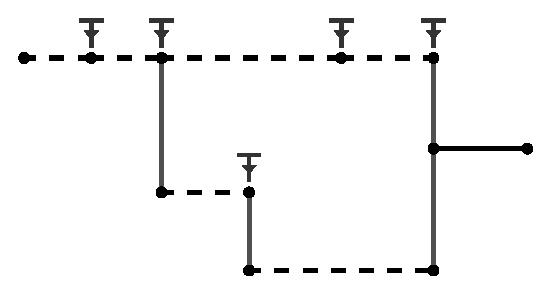
\includegraphics[width=0.45\textwidth]{images/event.eps}
    \caption{An example of event-driven score}
    \label{fig.event}
\end{figure}
Event-driven, or asynchronous design is a softwar design 
paradigm that is centered on the notion of asynchronous 
communication between different parts of the software.
This is commonly used when doing networked operations.

Instead of writing : 
\verb|play A; play B; play C|, in event-driven programming, one would write :
\begin{lstlisting}
when A is triggered
    play B
when B is triggered
    play C    
play A
\end{lstlisting}

Since i-score supports interactive events, one can easily write such event chaining.
An example is given in fig.~\ref{fig.event}. 
The advantage is that ordered operations can be written easily : there is no 
possibility for B to happen before A if there is a time constraint between A and B.
However, the execution engine will introduce a delay of one tick between each call.
The tick rate can be set to as low as one kilo-hertz.
\subsection{Simulating functions}
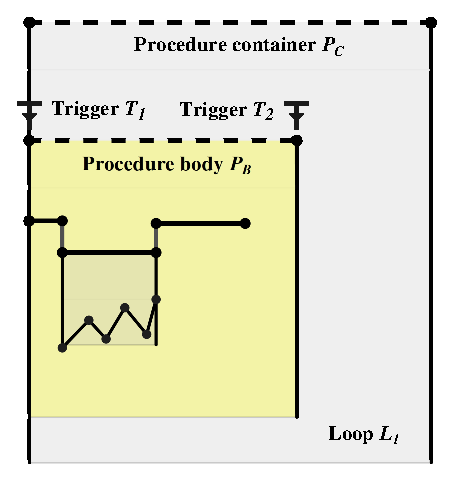
\includegraphics[width=0.45\textwidth]{images/function.eps}

% \subsection{References ?}

\section{Musical examples}\label{sec:typeset_text}

\subsection{Klavierstück}\label{subsec:body}
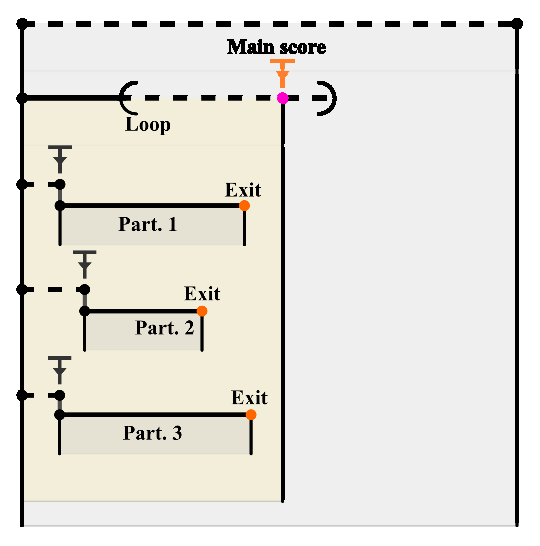
\includegraphics[width=0.45\textwidth]{images/partition.eps}

\subsection{Fibonacci recursive}

\section{Conclusion}
- plug-in architecture
- open-source
- soon : audio and midi support (midi can be done today with osc wrappers
but a piano-roll or sheet music view would be nice)
- computation graph may be useful to plug the input of a box 
to an output without using the tree
- other features : spatial, etc.
- embeddable 
- problématique de déboguage, analyse statique
\begin{acknowledgments}
    This work was funded by Blue Yeti and ANR.
\end{acknowledgments} 

\bibliography{icmc2016template}

\end{document}
